\documentclass[serif]{beamer}

\def\gridopacity{100}
\def\gridopacity{0}

% what is this for?
\usepackage{multimedia}

% see http://tex.stackexchange.com/a/24491
% for how to use enumitem with beamer
\usepackage{enumitem}
\setitemize{label=\usebeamerfont*{itemize item}%
  \usebeamercolor[fg]{itemize item}
  \usebeamertemplate{itemize item}}

% default page size is:
% \beamer@paperwidth 12.80cm%
% \beamer@paperheight 9.60cm%

\setbeamersize{text margin left=0.4cm,text margin right=0.4cm}

\usepackage{tikz}
\usetikzlibrary{calc,decorations.pathreplacing,positioning}
\usepackage{pgfplots}

\usepackage[clock,misc]{ifsym} % for \showclock

% pretty tables
\usepackage{multirow}
\usepackage{booktabs}

% this is from http://tex.stackexchange.com/a/103691
% taken from manual
\makeatletter
\pgfdeclareshape{document}{
\inheritsavedanchors[from=rectangle] % this is nearly a rectangle
\inheritanchorborder[from=rectangle]
\inheritanchor[from=rectangle]{center}
\inheritanchor[from=rectangle]{north}
\inheritanchor[from=rectangle]{south}
\inheritanchor[from=rectangle]{west}
\inheritanchor[from=rectangle]{east}
% ... and possibly more
\backgroundpath{% this is new
% store lower right in xa/ya and upper right in xb/yb
\southwest \pgf@xa=\pgf@x \pgf@ya=\pgf@y
\northeast \pgf@xb=\pgf@x \pgf@yb=\pgf@y
% compute corner of ‘‘flipped page’’
\pgf@xc=\pgf@xb \advance\pgf@xc by-5pt % this should be a parameter
\pgf@yc=\pgf@yb \advance\pgf@yc by-5pt
% construct main path
\pgfpathmoveto{\pgfpoint{\pgf@xa}{\pgf@ya}}
\pgfpathlineto{\pgfpoint{\pgf@xa}{\pgf@yb}}
\pgfpathlineto{\pgfpoint{\pgf@xc}{\pgf@yb}}
\pgfpathlineto{\pgfpoint{\pgf@xb}{\pgf@yc}}
\pgfpathlineto{\pgfpoint{\pgf@xb}{\pgf@ya}}
\pgfpathclose
% add little corner
\pgfpathmoveto{\pgfpoint{\pgf@xc}{\pgf@yb}}
\pgfpathlineto{\pgfpoint{\pgf@xc}{\pgf@yc}}
\pgfpathlineto{\pgfpoint{\pgf@xb}{\pgf@yc}}
\pgfpathlineto{\pgfpoint{\pgf@xc}{\pgf@yc}}
}
}
\makeatother

\usepackage{algorithm}
\usepackage[noend]{algpseudocode}

% symbols
\usepackage{amsmath} % assumes amsmath package installed
\usepackage{amssymb} % for \square
% non-italicized math subscripts
\newcommand{\ms}[1]{\mbox{\scriptsize #1}}
% from http://tex.stackexchange.com/a/5255
\DeclareMathOperator*{\argmin}{arg\,min}

% fonts
\renewcommand\rmdefault{pplx}
\renewcommand\mathfamilydefault{cmr}

\setbeamertemplate{navigation symbols}{}

\setbeamertemplate{footline}{%
   \raisebox{7pt}{\makebox[\paperwidth]{%
   \hfill\makebox[10pt]{\textcolor{gray}{%
   \small\insertframenumber\hspace{0.1in}}}}}}

\title{Pathfinding with Expensive Edge Evaluations: \\
Lazy Best-First Path Search with Edge Selectors}
%\author{Christopher M. Dellin and Siddhartha S. Srinivasa}
%\date{June 15, 2016}

\begin{document}

\begin{frame}[plain]
   %\begin{columns}
   %   \column{1.2\textwidth}
      \maketitle
   %\end{columns}
\end{frame}

%\begin{frame}
%   \frametitle{Pathfinding on Graphs}
%   
%   The \emph{shortest-path problem} is prevalent and fundamental.
%   
%   Lots of applications.
%   
%   Graph $G=(V,E)$, edge weight function $w: E \rightarrow \mathbb{R}$.
%   
%   Single-pair, all-pairs, single-source/single-sink, etc.
%   
%   Bounded-suboptimal, incremental, anytime, etc ...
%\end{frame}

\begin{frame}
   \frametitle{The Shortest Path Problem}
   \begin{tikzpicture}[font=\small]
      \tikzset{>=latex} % arrow heads
   
      \draw[step=1,black!15,very thin,opacity=\gridopacity] (0,0) grid (12,8);
      
      \only<2->{
         \node at (1,7) {\includegraphics[width=1.5cm]{figs/rubik.png}};
         \node at (3,7) {\includegraphics[width=1.5cm]{figs/15puzzle.png}};
      }
      \only<3->{
         \node at (5,7) {\includegraphics[width=1.5cm]{figs/internet-routers.jpg}};
      }
      \only<4->{
         \node[draw,align=center] at (7,7) {Optimal\\Motion\\Planning};
      }
      \only<5->{
         \node[draw,align=center] at (9,7) {Kino-\\Dynamic\\Planning};
      }
      \only<6->{
         \node[draw,align=center] at (11,7) {Convoy\\Routing};
      }
      
      \only<7->{
         % graph
         
         \coordinate (va) at ( 2.0,4.0);
         \coordinate (vb) at ( 3.5,4.7);
         \coordinate (vc) at ( 4.0,6.0);
         \coordinate (vd) at ( 5.5,4.5);
         \coordinate (ve) at ( 8.0,5.0);
         \coordinate (vf) at (10.0,4.0);
         \coordinate (vg) at ( 1.5,5.0);
         \coordinate (vh) at ( 4.0,3.5);
         \coordinate (vi) at ( 7.0,3.2);
         \coordinate (vj) at ( 6.5,5.5);
         \coordinate (vk) at ( 9.0,3.5);
         
         \only<10->{
            \node[circle,fill=black!20,inner sep=0.1cm] at (va) {};
            \node[circle,fill=black!20,inner sep=0.1cm] at (vf) {};
         }
         
         \only<11->{
            \draw[line width=0.2cm,color=black!30,line cap=round]
               (va) -- (vb) -- (vd) -- (ve) -- (vf);
         }
         
         \node[circle,fill=black,inner sep=0.05cm] at (va) {};
         \node[circle,fill=black,inner sep=0.05cm] at (vb) {};
         \node[circle,fill=black,inner sep=0.05cm] at (vc) {};
         \node[circle,fill=black,inner sep=0.05cm] at (vd) {};
         \node[circle,fill=black,inner sep=0.05cm] at (ve) {};
         \node[circle,fill=black,inner sep=0.05cm] at (vf) {};
         \node[circle,fill=black,inner sep=0.05cm] at (vg) {};
         \node[circle,fill=black,inner sep=0.05cm] at (vh) {};
         \node[circle,fill=black,inner sep=0.05cm] at (vi) {};
         \node[circle,fill=black,inner sep=0.05cm] at (vj) {};
         \node[circle,fill=black,inner sep=0.05cm] at (vk) {};
         
         \draw (va) -- (vb) coordinate [midway] (eab);
         \draw (vb) -- (vc) coordinate [midway] (ebc);
         \draw (vb) -- (vd) coordinate [midway] (ebd);
         \draw (vc) -- (vd) coordinate [midway] (ecd);
         \draw (vd) -- (ve) coordinate [midway] (ede);
         \draw (ve) -- (vf) coordinate [midway] (eef);
         \draw (va) -- (vg) coordinate [midway] (eag);
         \draw (vb) -- (vg) coordinate [midway] (ebg);
         \draw (va) -- (vh) coordinate [midway] (eah);
         \draw (vd) -- (vh) coordinate [midway] (edh);
         \draw (vb) -- (vh) coordinate [midway] (ebh);
         \draw (vd) -- (vi) coordinate [midway] (edi);
         \draw (ve) -- (vi) coordinate [midway] (eei);
         \draw (vc) -- (vj) coordinate [midway] (ecj);
         \draw (vd) -- (vj) coordinate [midway] (edj);
         \draw (ve) -- (vj) coordinate [midway] (eej);
         \draw (vf) -- (vk) coordinate [midway] (efk);
         \draw (vi) -- (vk) coordinate [midway] (eik);
         \draw (ve) -- (vk) coordinate [midway] (eek);
         
         \only<8->{
            \node[circle,inner sep=0.02cm,fill=white,opacity=0.9,font=\scriptsize] at (eab) {5};
            \node[circle,inner sep=0.02cm,fill=white,opacity=0.9,font=\scriptsize] at (ebc) {5};
            \node[circle,inner sep=0.02cm,fill=white,opacity=0.9,font=\scriptsize] at (ebd) {6};
            \node[circle,inner sep=0.02cm,fill=white,opacity=0.9,font=\scriptsize] at (ecd) {7};
            \node[circle,inner sep=0.02cm,fill=white,opacity=0.9,font=\scriptsize] at (ede) {9};
            \node[circle,inner sep=0.02cm,fill=white,opacity=0.9,font=\scriptsize] at (eef) {7};
            \node[circle,inner sep=0.02cm,fill=white,opacity=0.9,font=\scriptsize] at (eag) {3};
            \node[circle,inner sep=0.02cm,fill=white,opacity=0.9,font=\scriptsize] at (ebg) {6};
            \node[circle,inner sep=0.02cm,fill=white,opacity=0.9,font=\scriptsize] at (eah) {6};
            \node[circle,inner sep=0.02cm,fill=white,opacity=0.9,font=\scriptsize] at (edh) {7};
            \node[circle,inner sep=0.02cm,fill=white,opacity=0.9,font=\scriptsize] at (ebh) {5};
            \node[circle,inner sep=0.02cm,fill=white,opacity=0.9,font=\scriptsize] at (edi) {8};
            \node[circle,inner sep=0.02cm,fill=white,opacity=0.9,font=\scriptsize] at (eei) {8};
            \node[circle,inner sep=0.02cm,fill=white,opacity=0.9,font=\scriptsize] at (ecj) {8};
            \node[circle,inner sep=0.02cm,fill=white,opacity=0.9,font=\scriptsize] at (edj) {6};
            \node[circle,inner sep=0.02cm,fill=white,opacity=0.9,font=\scriptsize] at (eej) {4};
            \node[circle,inner sep=0.02cm,fill=white,opacity=0.9,font=\scriptsize] at (efk) {3};
            \node[circle,inner sep=0.02cm,fill=white,opacity=0.9,font=\scriptsize] at (eik) {6};
            \node[circle,inner sep=0.02cm,fill=white,opacity=0.9,font=\scriptsize] at (eek) {6};
         }
      }
      
      \only<7->{
         \node[draw,align=center,minimum height=1.0cm,minimum width=2.9cm,thick]
            at (4.0,2.05) {Graph\\$G=(V,E)$};
      }
      \only<8->{
         \node[draw,align=center,minimum height=1.0cm,minimum width=2.9cm,thick]
            at (8.0,2.05) {Weight Function\\$w:E \rightarrow \mathbb{R}$};
         \node[align=center,color=black!50] at (10.75,2) {
            $w(e) \geq 0$\\
            $w(e) > 0$\\
            $w(e) \geq w_{\ms{est}}(e)$\\
         };
      }
      \only<9->{
         \node[draw,align=center,minimum height=1.0cm,minimum width=4cm,thick]
            (alg) at (6,0.55) {Shortest Path\\Algorithm};
         \draw[->] (4.5,1.55) -- (4.5,1.05);
         \draw[->] (7.5,1.55) -- (7.5,1.05);
      }
      \only<10->{
         \node[draw,align=center,shape=document,minimum width=3.0cm,ultra thin]
            (query) at (2,0.55) {Query $v_s$, $v_t$\;\;};
         \draw[->] (query.east) -- (alg.west);
         \node[left=0.1cm of va] {$v_s$};
         \node[right=0.1cm of vf] {$v_t$};
      }
      \only<11->{
         \node[draw,align=center,shape=document,minimum width=2.0cm,ultra thin]
            (path) at (10,0.55) {Path $p^*$\;};
         \draw[->] (alg.east) -- (path.west);
      }
      
   \end{tikzpicture}
\end{frame}

% application     -> graph representation    -> algorithm      -> path -> application solution
% [ lots of them]    G=(V,E)                    [lots of them]
%                    w: e -> R
%                    root vertices (v_s, v_t)
%                    (vertex heuristic?)
%                    problem
%                    - single-pair
%                    - optimal
%                    - bounded-suboptimal
%                    - bounded-cost
 
%\begin{frame}
%   \frametitle{Pathfinding on Graphs 2}
%   \begin{tikzpicture}
%      \tikzset{>=latex} % arrow heads
%   
%      \draw[step=1,black!15,very thin,opacity=\gridopacity] (0,0) grid (12,8);
%      
%      \node at (1.5,7.5) {Applications};
%      
%      \node at (1.0,6.5) {\includegraphics[width=1.5cm]{figs/rubik.png}};
%      \node at (2.0,6.5) {\includegraphics[width=1.5cm]{figs/15puzzle.png}};
%      \node at (1.5,4.5) {\includegraphics[width=1.5cm]{figs/internet-routers.jpg}};
%      \node at (1.5,3.0) {Traffic Routing};
%      \node at (1.5,2.5) {Motion Planning};
%      %\node at (1.5,2.0) {Optimal Motion Planning};
%      
%      \node at (6.0,7.5) {Representation};
%      
%      \node at (10.5,7.5) {Algorithms};
%      
%      \node[align=center] at (7,3) {
%         $w(e) \geq 0$\\
%         $w(e) > 0$\\
%         $w(e) \geq w_{\ms{est}}(e)$\\
%      };
%      
%      %\draw[step=1cm,black!10,very thin] (0,0) grid (8,4);
%      \node[draw,align=center,minimum height=1.0cm,thick]
%         at (6.0,6.0) {Graph\\$G=(V,E)$};
%      \node[draw,align=center,minimum height=1.0cm,thick]
%         at (6.0,4.5) {Weight Function\\$w:E \rightarrow [0,+\infty]$};
%      \node[draw,align=center,shape=document,minimum width=3.0cm,ultra thin]
%         (query) at (6,1) {Query $v_s$, $v_t$\;\;};
%      
%      \node at (10.5,6.5) {Dijkstra's};
%      \node at (10.5,5.5) {A*};
%      \node at (10.5,4.5) {IDA*};
%      \node at (10.5,3.5) {PEA*};
%      
%   \end{tikzpicture}
%\end{frame}

\begin{frame}
   \frametitle{The Shortest Path Problem}
   \begin{tikzpicture}[font=\small]
      \tikzset{>=latex} % arrow heads
      
      \draw[step=1,black!15,very thin,opacity=\gridopacity] (0,0) grid (12,8);
   
      % highlight puzzles
      \only<2-4>{
         \fill[blue!20,rounded corners] (0.1,6.1) rectangle (3.9,7.9);
      }
      
      % highlight motion planning
      \only<5-9>{
         \fill[blue!20,rounded corners] (6.1,6.1) rectangle (7.9,7.9);
         \only<6->{
            \node[align=center,font=\scriptsize] at (11.0,5.0) {Configuration\\Space};
         }
      }
      
      % highlight kinodynamic planning
      \only<10-11>{
         \fill[blue!20,rounded corners] (8.1,6.1) rectangle (9.9,7.9);
         \node[align=center,font=\scriptsize] at (11.0,5.0) {Kinodynamic\\State Space};
      }
      
      % highlight convoy
      \only<12->{
         \fill[blue!20,rounded corners] (10.1,6.1) rectangle (11.9,7.9);
         \only<14->{
            \node[draw,align=center,font=\scriptsize] (satnode) at (11.0,5.5) {Satellite};
         }
      }
   
      % c-space obstacles
      \only<8-11>{
         \fill[black!20] (4.5,3.25) rectangle (6.0,5.0);
         \fill[black!20] (8.5,4.00) rectangle (9.5,5.5);
         \only<8-9>{
            \node[color=black!70,font=\scriptsize] at (5.25,3.5) {$CO_1$};
            \node[color=black!70,font=\scriptsize] at (9.0,5.25) {$CO_2$};
         }
         \only<10->{
            \node[color=black!70,font=\scriptsize] at (5.25,3.5) {$SO_1$};
            \node[color=black!70,font=\scriptsize] at (9.0,5.25) {$SO_2$};
         }
      }
      
      % graph start
      \coordinate (va) at ( 2.0,4.0);
      \coordinate (vb) at ( 3.5,4.7);
      \coordinate (vc) at ( 4.0,6.0);
      \coordinate (vd) at ( 5.5,4.5);
      \coordinate (ve) at ( 8.0,5.0);
      \coordinate (vf) at (10.0,4.0);
      \coordinate (vg) at ( 1.5,5.0);
      \coordinate (vh) at ( 4.0,3.5);
      \coordinate (vi) at ( 7.0,3.2);
      \coordinate (vj) at ( 6.5,5.5);
      \coordinate (vk) at ( 9.0,3.5);
      
      %\node[circle,fill=black!20,inner sep=0.1cm] at (va) {};
      %\node[circle,fill=black!20,inner sep=0.1cm] at (vf) {};
      
      \node[circle,fill=black,inner sep=0.05cm] at (va) {};
      \node[circle,fill=black,inner sep=0.05cm] at (vb) {};
      \node[circle,fill=black,inner sep=0.05cm] at (vc) {};
      \node[circle,fill=black,inner sep=0.05cm] at (vd) {};
      \node[circle,fill=black,inner sep=0.05cm] at (ve) {};
      \node[circle,fill=black,inner sep=0.05cm] at (vf) {};
      \node[circle,fill=black,inner sep=0.05cm] at (vg) {};
      \node[circle,fill=black,inner sep=0.05cm] at (vh) {};
      \node[circle,fill=black,inner sep=0.05cm] at (vi) {};
      \node[circle,fill=black,inner sep=0.05cm] at (vj) {};
      \node[circle,fill=black,inner sep=0.05cm] at (vk) {};
      
      \draw (va) -- (vb) coordinate [midway] (eab);
      \draw (vb) -- (vc) coordinate [midway] (ebc);
      \draw (vb) -- (vd) coordinate [midway] (ebd);
      \draw (vc) -- (vd) coordinate [midway] (ecd);
      \draw (vd) -- (ve) coordinate [midway] (ede);
      \draw (ve) -- (vf) coordinate [midway] (eef);
      \draw (va) -- (vg) coordinate [midway] (eag);
      \draw (vb) -- (vg) coordinate [midway] (ebg);
      \draw (va) -- (vh) coordinate [midway] (eah);
      \draw (vd) -- (vh) coordinate [midway] (edh);
      \draw (vb) -- (vh) coordinate [midway] (ebh);
      \draw (vd) -- (vi) coordinate [midway] (edi);
      \draw (ve) -- (vi) coordinate [midway] (eei);
      \draw (vc) -- (vj) coordinate [midway] (ecj);
      \draw (vd) -- (vj) coordinate [midway] (edj);
      \draw (ve) -- (vj) coordinate [midway] (eej);
      \draw (vf) -- (vk) coordinate [midway] (efk);
      \draw (vi) -- (vk) coordinate [midway] (eik);
      \draw (ve) -- (vk) coordinate [midway] (eek);
      
      \only<4-4>{
         \node[circle,inner sep=0.02cm,fill=white,opacity=0.9,font=\scriptsize] at (eab) {1};
         \node[circle,inner sep=0.02cm,fill=white,opacity=0.9,font=\scriptsize] at (ebc) {1};
         \node[circle,inner sep=0.02cm,fill=white,opacity=0.9,font=\scriptsize] at (ebd) {1};
         \node[circle,inner sep=0.02cm,fill=white,opacity=0.9,font=\scriptsize] at (ecd) {1};
         \node[circle,inner sep=0.02cm,fill=white,opacity=0.9,font=\scriptsize] at (ede) {1};
         \node[circle,inner sep=0.02cm,fill=white,opacity=0.9,font=\scriptsize] at (eef) {1};
         \node[circle,inner sep=0.02cm,fill=white,opacity=0.9,font=\scriptsize] at (eag) {1};
         \node[circle,inner sep=0.02cm,fill=white,opacity=0.9,font=\scriptsize] at (ebg) {1};
         \node[circle,inner sep=0.02cm,fill=white,opacity=0.9,font=\scriptsize] at (eah) {1};
         \node[circle,inner sep=0.02cm,fill=white,opacity=0.9,font=\scriptsize] at (edh) {1};
         \node[circle,inner sep=0.02cm,fill=white,opacity=0.9,font=\scriptsize] at (ebh) {1};
         \node[circle,inner sep=0.02cm,fill=white,opacity=0.9,font=\scriptsize] at (edi) {1};
         \node[circle,inner sep=0.02cm,fill=white,opacity=0.9,font=\scriptsize] at (eei) {1};
         \node[circle,inner sep=0.02cm,fill=white,opacity=0.9,font=\scriptsize] at (ecj) {1};
         \node[circle,inner sep=0.02cm,fill=white,opacity=0.9,font=\scriptsize] at (edj) {1};
         \node[circle,inner sep=0.02cm,fill=white,opacity=0.9,font=\scriptsize] at (eej) {1};
         \node[circle,inner sep=0.02cm,fill=white,opacity=0.9,font=\scriptsize] at (efk) {1};
         \node[circle,inner sep=0.02cm,fill=white,opacity=0.9,font=\scriptsize] at (eik) {1};
         \node[circle,inner sep=0.02cm,fill=white,opacity=0.9,font=\scriptsize] at (eek) {1};
      }
      
      % motion planning
      \only<7-8>{
         \node[circle,inner sep=0.02cm,fill=white,opacity=0.9,font=\scriptsize] at (eab) {5};
         \node[circle,inner sep=0.02cm,fill=white,opacity=0.9,font=\scriptsize] at (ebc) {5};
         \node[circle,inner sep=0.02cm,fill=white,opacity=0.9,font=\scriptsize] at (ebd) {6};
         \node[circle,inner sep=0.02cm,fill=white,opacity=0.9,font=\scriptsize] at (ecd) {7};
         \node[circle,inner sep=0.02cm,fill=white,opacity=0.9,font=\scriptsize] at (ede) {9};
         \node[circle,inner sep=0.02cm,fill=white,opacity=0.9,font=\scriptsize] at (eef) {7};
         \node[circle,inner sep=0.02cm,fill=white,opacity=0.9,font=\scriptsize] at (eag) {3};
         \node[circle,inner sep=0.02cm,fill=white,opacity=0.9,font=\scriptsize] at (ebg) {6};
         \node[circle,inner sep=0.02cm,fill=white,opacity=0.9,font=\scriptsize] at (eah) {6};
         \node[circle,inner sep=0.02cm,fill=white,opacity=0.9,font=\scriptsize] at (edh) {7};
         \node[circle,inner sep=0.02cm,fill=white,opacity=0.9,font=\scriptsize] at (ebh) {5};
         \node[circle,inner sep=0.02cm,fill=white,opacity=0.9,font=\scriptsize] at (edi) {8};
         \node[circle,inner sep=0.02cm,fill=white,opacity=0.9,font=\scriptsize] at (eei) {8};
         \node[circle,inner sep=0.02cm,fill=white,opacity=0.9,font=\scriptsize] at (ecj) {8};
         \node[circle,inner sep=0.02cm,fill=white,opacity=0.9,font=\scriptsize] at (edj) {6};
         \node[circle,inner sep=0.02cm,fill=white,opacity=0.9,font=\scriptsize] at (eej) {4};
         \node[circle,inner sep=0.02cm,fill=white,opacity=0.9,font=\scriptsize] at (efk) {3};
         \node[circle,inner sep=0.02cm,fill=white,opacity=0.9,font=\scriptsize] at (eik) {6};
         \node[circle,inner sep=0.02cm,fill=white,opacity=0.9,font=\scriptsize] at (eek) {6};
      }
      \only<9-11>{
         \node[circle,inner sep=0.02cm,fill=white,opacity=0.9,font=\scriptsize] at (eab) {5};
         \node[circle,inner sep=0.02cm,fill=white,opacity=0.9,font=\scriptsize] at (ebc) {5};
         \node[circle,inner sep=0.02cm,fill=white,opacity=0.9,font=\scriptsize] at (ebd) {$\infty$};
         \node[circle,inner sep=0.02cm,fill=white,opacity=0.9,font=\scriptsize] at (ecd) {$\infty$};
         \node[circle,inner sep=0.02cm,fill=white,opacity=0.9,font=\scriptsize] at (ede) {$\infty$};
         \node[circle,inner sep=0.02cm,fill=white,opacity=0.9,font=\scriptsize] at (eef) {$\infty$};
         \node[circle,inner sep=0.02cm,fill=white,opacity=0.9,font=\scriptsize] at (eag) {3};
         \node[circle,inner sep=0.02cm,fill=white,opacity=0.9,font=\scriptsize] at (ebg) {6};
         \node[circle,inner sep=0.02cm,fill=white,opacity=0.9,font=\scriptsize] at (eah) {6};
         \node[circle,inner sep=0.02cm,fill=white,opacity=0.9,font=\scriptsize] at (edh) {$\infty$};
         \node[circle,inner sep=0.02cm,fill=white,opacity=0.9,font=\scriptsize] at (ebh) {5};
         \node[circle,inner sep=0.02cm,fill=white,opacity=0.9,font=\scriptsize] at (edi) {$\infty$};
         \node[circle,inner sep=0.02cm,fill=white,opacity=0.9,font=\scriptsize] at (eei) {8};
         \node[circle,inner sep=0.02cm,fill=white,opacity=0.9,font=\scriptsize] at (ecj) {8};
         \node[circle,inner sep=0.02cm,fill=white,opacity=0.9,font=\scriptsize] at (edj) {$\infty$};
         \node[circle,inner sep=0.02cm,fill=white,opacity=0.9,font=\scriptsize] at (eej) {4};
         \node[circle,inner sep=0.02cm,fill=white,opacity=0.9,font=\scriptsize] at (efk) {3};
         \node[circle,inner sep=0.02cm,fill=white,opacity=0.9,font=\scriptsize] at (eik) {6};
         \node[circle,inner sep=0.02cm,fill=white,opacity=0.9,font=\scriptsize] at (eek) {$\infty$};
      }
      
      % convoy
      \only<13->{
         \node[circle,inner sep=0.02cm,fill=white,opacity=0.9,font=\scriptsize] at (eab) {?};
         \node[circle,inner sep=0.02cm,fill=white,opacity=0.9,font=\scriptsize] at (ebc) {?};
         \node[circle,inner sep=0.02cm,fill=white,opacity=0.9,font=\scriptsize] at (ebd) {?};
         \node[circle,inner sep=0.02cm,fill=white,opacity=0.9,font=\scriptsize] at (ecd) {?};
         \node[circle,inner sep=0.02cm,fill=white,opacity=0.9,font=\scriptsize] at (ede) {?};
         \node[circle,inner sep=0.02cm,fill=white,opacity=0.9,font=\scriptsize] at (eef) {?};
         \node[circle,inner sep=0.02cm,fill=white,opacity=0.9,font=\scriptsize] at (eag) {?};
         \node[circle,inner sep=0.02cm,fill=white,opacity=0.9,font=\scriptsize] at (ebg) {?};
         \node[circle,inner sep=0.02cm,fill=white,opacity=0.9,font=\scriptsize] at (eah) {?};
         \node[circle,inner sep=0.02cm,fill=white,opacity=0.9,font=\scriptsize] at (edh) {?};
         \node[circle,inner sep=0.02cm,fill=white,opacity=0.9,font=\scriptsize] at (ebh) {?};
         %\node[circle,inner sep=0.02cm,fill=white,opacity=0.9,font=\scriptsize] at (edi) {?};
         \node[circle,inner sep=0.02cm,fill=white,opacity=0.9,font=\scriptsize] at (eei) {?};
         \node[circle,inner sep=0.02cm,fill=white,opacity=0.9,font=\scriptsize] at (ecj) {?};
         \node[circle,inner sep=0.02cm,fill=white,opacity=0.9,font=\scriptsize] at (edj) {?};
         \node[circle,inner sep=0.02cm,fill=white,opacity=0.9,font=\scriptsize] at (eej) {?};
         \node[circle,inner sep=0.02cm,fill=white,opacity=0.9,font=\scriptsize] at (efk) {?};
         \node[circle,inner sep=0.02cm,fill=white,opacity=0.9,font=\scriptsize] at (eik) {?};
         % first uncover
         \only<13-14>{\node[circle,inner sep=0.02cm,fill=white,opacity=0.9,font=\scriptsize] at (eek) {?};}
         \only<15->{  \node[circle,inner sep=0.02cm,fill=white,opacity=0.9,font=\scriptsize] (sateek) at (eek) {7.8};}
         \only<15>{\draw[ultra thick,red,->] (satnode.south west) -- (sateek.east);}
         % second uncover
         \only<13-15>{\node[circle,inner sep=0.02cm,fill=white,opacity=0.9,font=\scriptsize] at (edi) {?};}
         \only<16->{  \node[circle,inner sep=0.02cm,fill=white,opacity=0.9,font=\scriptsize] (satedi) at (edi) {$\infty$};}
         \only<16>{\draw[ultra thick,red,->] (satnode.south west) -- (satedi.east);}
      }

      %\node[left=0.1cm of va] {$v_s$};
      %\node[right=0.1cm of vf] {$v_t$};
      
      %\fill[white,opacity=0.8] (0,3) rectangle (12,6.5);
      % graph end
      
      \node[draw,thick,minimum height=1.5cm,minimum width=5.5cm,anchor=north] at (3,2.9) {};
      \node [anchor=north] at (3,2.9) {\begin{minipage}{5cm}
         \begin{center}
         Graph $G=(V,E)$:
         \end{center}
         \vspace{-0.4cm}
         
         % puzzles
         \only<3-4>{
            $v:$ puzzle state; $|V| = 10^{15}$
            
            $e:$ puzzle move
         }
         
         % highlight motion planning
         \only<6-9>{
            $v:$ arm configuration; $|V| \approx 10^{5}$
         
            $e:$ arm motion
         }
      \end{minipage}};
   
      \node[draw,thick,minimum height=1.5cm,minimum width=5.5cm,anchor=north] at (9,2.9) {};
      \node [anchor=north] at (9,2.9) {\begin{minipage}{5cm}
         \begin{center}
         Weight Function $w:E \rightarrow \mathbb{R}$:
         \end{center}
         \vspace{-0.4cm}
      
         % puzzles
         \only<4-4>{
            $w(e) = 1 \; \forall e \in E$
         }
         
         % highlight motion planning
         \only<7-8>{%
            $w(e) = \left\{ \arraycolsep=2pt \begin{array}{cl}
            ||e|| & \mbox{if $e$ collision-free} \\
            & \\
            \end{array} \right.$
         }%
         \only<9-9>{%
            $w(e) = \left\{ \arraycolsep=2pt \begin{array}{cl}
            ||e|| & \mbox{if $e$ collision-free} \\
            \infty & \mbox{otherwise} \\
            \end{array} \right.$
         }%
         \only<11-11>{%
            \vspace{0.2cm}
            $w(e) = \mbox{2P-BVP}(q_a, q_b)$
         }%
         \only<14->{%
            \vspace{0.2cm}
            $w(e) = \mbox{Reconnaisance}(e)$
         }%
      \end{minipage}};
   
      \node at (1,7) {\includegraphics[width=1.5cm]{figs/rubik.png}};
      \node at (3,7) {\includegraphics[width=1.5cm]{figs/15puzzle.png}};
      \node at (5,7) {\includegraphics[width=1.5cm]{figs/internet-routers.jpg}};
      \node[draw,align=center] at (7,7) {Optimal\\Motion\\Planning};
      \node[draw,align=center] at (9,7) {Kino-\\Dynamic\\Planning};
      \node[draw,align=center] at (11,7) {Convoy\\Routing};
      
      \node[draw,align=center,minimum height=1.0cm,minimum width=4cm,thick]
         (alg) at (6,0.55) {Shortest Path\\Algorithm};
      \draw[->] (4.5,1.40) -- (4.5,1.05);
      \draw[->] (7.5,1.40) -- (7.5,1.05);
      \node[draw,align=center,shape=document,minimum width=3.0cm,ultra thin]
         (query) at (2,0.55) {Query $v_s$, $v_t$\;\;};
      \draw[->] (query.east) -- (alg.west);
      \node[draw,align=center,shape=document,minimum width=2.0cm,ultra thin]
         (path) at (10,0.55) {Path $p^*$\;};
      \draw[->] (alg.east) -- (path.west);
   
   \end{tikzpicture}
\end{frame}

\begin{frame}
   \frametitle{Pathfinding with Expensive Edge Evaluations}
   
   In some domains, determining edge weights\\
   is a computationally expensive operation.
   
   \pause
   \vspace{0.4cm}
   \emph{Question: How can we solve shortest-path problems\\
      \quad \quad \quad \quad \, while reducing the number of edges evaluated?}
   
   \pause
   \vspace{0.4cm}
   Outline of talk:
   \begin{itemize}
   \pause
   \item Review of lazy search approaches
   \pause
   \item LazySP algorithm outline (using \emph{edge selectors})
   \pause
   \item Equivalence to existing algorithms
   \pause
   \item Novel edge selectors
   \pause
   \item Experimental results
   \end{itemize}
\end{frame}

\begin{frame}
   \frametitle{Review of Prior Approaches}
   
   \begin{tikzpicture}[font=\small]
      \tikzset{>=latex} % arrow heads
      
      \draw[step=1,black!15,very thin,opacity=\gridopacity] (0,0) grid (12,8);
      
      % graph start
      \coordinate (va) at ( 2.0,5.6);
      \coordinate (vb) at ( 3.5,6.3);
      \coordinate (vc) at ( 4.0,7.6);
      \coordinate (vd) at ( 5.5,6.1);
      \coordinate (ve) at ( 8.0,6.6);
      \coordinate (vf) at (10.0,5.6);
      \coordinate (vg) at ( 1.5,6.6);
      \coordinate (vh) at ( 4.0,5.1);
      \coordinate (vi) at ( 7.0,4.8);
      \coordinate (vj) at ( 6.5,7.1);
      \coordinate (vk) at ( 9.0,5.1);
      
      % start/goal highlighting
      \node[circle,fill=black!20,inner sep=0.1cm] at (va) {};
      \node[circle,fill=black!20,inner sep=0.1cm] at (vf) {};
      
      % edges, grey
      \only<1-2,4,10>{
         \draw[black!30] (va) -- (vb) coordinate [midway] (eab);
         \draw[black!30] (vb) -- (vc) coordinate [midway] (ebc);
         \draw[black!30] (vb) -- (vd) coordinate [midway] (ebd);
         \draw[black!30] (vc) -- (vd) coordinate [midway] (ecd);
         \draw[black!30] (vd) -- (ve) coordinate [midway] (ede);
         \draw[black!30] (ve) -- (vf) coordinate [midway] (eef);
         \draw[black!30] (va) -- (vg) coordinate [midway] (eag);
         \draw[black!30] (vb) -- (vg) coordinate [midway] (ebg);
         \draw[black!30] (va) -- (vh) coordinate [midway] (eah);
         \draw[black!30] (vd) -- (vh) coordinate [midway] (edh);
         \draw[black!30] (vb) -- (vh) coordinate [midway] (ebh);
         \draw[black!30] (vd) -- (vi) coordinate [midway] (edi);
         \draw[black!30] (ve) -- (vi) coordinate [midway] (eei);
         \draw[black!30] (vc) -- (vj) coordinate [midway] (ecj);
         \draw[black!30] (vd) -- (vj) coordinate [midway] (edj);
         \draw[black!30] (ve) -- (vj) coordinate [midway] (eej);
         \draw[black!30] (vf) -- (vk) coordinate [midway] (efk);
         \draw[black!30] (vi) -- (vk) coordinate [midway] (eik);
         \draw[black!30] (ve) -- (vk) coordinate [midway] (eek);
         
         \node[circle,inner sep=0.02cm,fill=white,opacity=0.9,font=\scriptsize] at (eab) {?};
         \node[circle,inner sep=0.02cm,fill=white,opacity=0.9,font=\scriptsize] at (ebc) {?};
         \node[circle,inner sep=0.02cm,fill=white,opacity=0.9,font=\scriptsize] at (ebd) {?};
         \node[circle,inner sep=0.02cm,fill=white,opacity=0.9,font=\scriptsize] at (ecd) {?};
         \node[circle,inner sep=0.02cm,fill=white,opacity=0.9,font=\scriptsize] at (ede) {?};
         \node[circle,inner sep=0.02cm,fill=white,opacity=0.9,font=\scriptsize] at (eef) {?};
         \node[circle,inner sep=0.02cm,fill=white,opacity=0.9,font=\scriptsize] at (eag) {?};
         \node[circle,inner sep=0.02cm,fill=white,opacity=0.9,font=\scriptsize] at (ebg) {?};
         \node[circle,inner sep=0.02cm,fill=white,opacity=0.9,font=\scriptsize] at (eah) {?};
         \node[circle,inner sep=0.02cm,fill=white,opacity=0.9,font=\scriptsize] at (edh) {?};
         \node[circle,inner sep=0.02cm,fill=white,opacity=0.9,font=\scriptsize] at (ebh) {?};
         \node[circle,inner sep=0.02cm,fill=white,opacity=0.9,font=\scriptsize] at (edi) {?};
         \node[circle,inner sep=0.02cm,fill=white,opacity=0.9,font=\scriptsize] at (eei) {?};
         \node[circle,inner sep=0.02cm,fill=white,opacity=0.9,font=\scriptsize] at (ecj) {?};
         \node[circle,inner sep=0.02cm,fill=white,opacity=0.9,font=\scriptsize] at (edj) {?};
         \node[circle,inner sep=0.02cm,fill=white,opacity=0.9,font=\scriptsize] at (eej) {?};
         \node[circle,inner sep=0.02cm,fill=white,opacity=0.9,font=\scriptsize] at (efk) {?};
         \node[circle,inner sep=0.02cm,fill=white,opacity=0.9,font=\scriptsize] at (eik) {?};
         \node[circle,inner sep=0.02cm,fill=white,opacity=0.9,font=\scriptsize] at (eek) {?};
      }
      
      % edges, black
      \only<3>{
         \draw (va) -- (vb) coordinate [midway] (eab);
         \draw (vb) -- (vc) coordinate [midway] (ebc);
         \draw (vb) -- (vd) coordinate [midway] (ebd);
         \draw (vc) -- (vd) coordinate [midway] (ecd);
         \draw (vd) -- (ve) coordinate [midway] (ede);
         \draw (ve) -- (vf) coordinate [midway] (eef);
         \draw (va) -- (vg) coordinate [midway] (eag);
         \draw (vb) -- (vg) coordinate [midway] (ebg);
         \draw (va) -- (vh) coordinate [midway] (eah);
         \draw (vd) -- (vh) coordinate [midway] (edh);
         \draw (vb) -- (vh) coordinate [midway] (ebh);
         \draw (vd) -- (vi) coordinate [midway] (edi);
         \draw (ve) -- (vi) coordinate [midway] (eei);
         \draw (vc) -- (vj) coordinate [midway] (ecj);
         \draw (vd) -- (vj) coordinate [midway] (edj);
         \draw (ve) -- (vj) coordinate [midway] (eej);
         \draw (vf) -- (vk) coordinate [midway] (efk);
         \draw (vi) -- (vk) coordinate [midway] (eik);
         \draw (ve) -- (vk) coordinate [midway] (eek);
         
         \node[circle,inner sep=0.02cm,fill=white,opacity=0.9,font=\scriptsize] at (eab) {5};
         \node[circle,inner sep=0.02cm,fill=white,opacity=0.9,font=\scriptsize] at (ebc) {5};
         \node[circle,inner sep=0.02cm,fill=white,opacity=0.9,font=\scriptsize] at (ebd) {6};
         \node[circle,inner sep=0.02cm,fill=white,opacity=0.9,font=\scriptsize] at (ecd) {7};
         \node[circle,inner sep=0.02cm,fill=white,opacity=0.9,font=\scriptsize] at (ede) {9};
         \node[circle,inner sep=0.02cm,fill=white,opacity=0.9,font=\scriptsize] at (eef) {7};
         \node[circle,inner sep=0.02cm,fill=white,opacity=0.9,font=\scriptsize] at (eag) {3};
         \node[circle,inner sep=0.02cm,fill=white,opacity=0.9,font=\scriptsize] at (ebg) {6};
         \node[circle,inner sep=0.02cm,fill=white,opacity=0.9,font=\scriptsize] at (eah) {6};
         \node[circle,inner sep=0.02cm,fill=white,opacity=0.9,font=\scriptsize] at (edh) {7};
         \node[circle,inner sep=0.02cm,fill=white,opacity=0.9,font=\scriptsize] at (ebh) {5};
         \node[circle,inner sep=0.02cm,fill=white,opacity=0.9,font=\scriptsize] at (edi) {8};
         \node[circle,inner sep=0.02cm,fill=white,opacity=0.9,font=\scriptsize] at (eei) {8};
         \node[circle,inner sep=0.02cm,fill=white,opacity=0.9,font=\scriptsize] at (ecj) {8};
         \node[circle,inner sep=0.02cm,fill=white,opacity=0.9,font=\scriptsize] at (edj) {6};
         \node[circle,inner sep=0.02cm,fill=white,opacity=0.9,font=\scriptsize] at (eej) {4};
         \node[circle,inner sep=0.02cm,fill=white,opacity=0.9,font=\scriptsize] at (efk) {3};
         \node[circle,inner sep=0.02cm,fill=white,opacity=0.9,font=\scriptsize] at (eik) {6};
         \node[circle,inner sep=0.02cm,fill=white,opacity=0.9,font=\scriptsize] at (eek) {6};
      }
      
      % NEXT, A* stuff
      
      % OPEN list highlighting (A*)
      \only<5>{\node[circle,fill=blue!70,inner sep=0.15cm] at (va) {};}
      \only<6-9>{\node[circle,fill=black!40,inner sep=0.15cm] at (va) {};}
      \only<6>{\node[circle,fill=blue!70,inner sep=0.15cm] at (vb) {};}
      \only<7-9>{\node[circle,fill=black!40,inner sep=0.15cm] at (vb) {};}
      \only<6-9>{\node[circle,fill=blue!40,inner sep=0.15cm] at (vg) {};}
      \only<6>{\node[circle,fill=blue!40,inner sep=0.15cm] at (vh) {};}
      \only<7>{\node[circle,fill=blue!70,inner sep=0.15cm] at (vh) {};}
      \only<8-9>{\node[circle,fill=black!40,inner sep=0.15cm] at (vh) {};}
      \only<7>{\node[circle,fill=blue!40,inner sep=0.15cm] at (vc) {};}
      \only<8>{\node[circle,fill=blue!70,inner sep=0.15cm] at (vc) {};}
      \only<9>{\node[circle,fill=black!40,inner sep=0.15cm] at (vc) {};}
      \only<7-9>{\node[circle,fill=blue!40,inner sep=0.15cm] at (vd) {};}
      \only<9>{\node[circle,fill=blue!70,inner sep=0.15cm] at (vj) {};}
      
      % first expansion
      \only<5>{
         \draw[black!30] (va) -- (vb) node[midway,circle,inner sep=0.02cm,fill=white,opacity=0.9,font=\scriptsize] {?};
         \draw[black!30] (va) -- (vg) node[midway,circle,inner sep=0.02cm,fill=white,opacity=0.9,font=\scriptsize] {?};
         \draw[black!30] (va) -- (vh) node[midway,circle,inner sep=0.02cm,fill=white,opacity=0.9,font=\scriptsize] {?};
      }
      \only<6-9>{
         \draw[black] (va) -- (vb) node[midway,circle,inner sep=0.02cm,fill=white,opacity=0.9,font=\scriptsize] {5};
         \draw[black] (va) -- (vg) node[midway,circle,inner sep=0.02cm,fill=white,opacity=0.9,font=\scriptsize] {3};
         \draw[black] (va) -- (vh) node[midway,circle,inner sep=0.02cm,fill=white,opacity=0.9,font=\scriptsize] {6};
      }
      % second expansion
      \only<5-6>{
         \draw[black!30] (vb) -- (vc) node[midway,circle,inner sep=0.02cm,fill=white,opacity=0.9,font=\scriptsize] {?};
         \draw[black!30] (vb) -- (vd) node[midway,circle,inner sep=0.02cm,fill=white,opacity=0.9,font=\scriptsize] {?};
         \draw[black!30] (vb) -- (vg) node[midway,circle,inner sep=0.02cm,fill=white,opacity=0.9,font=\scriptsize] {?};
         \draw[black!30] (vb) -- (vh) node[midway,circle,inner sep=0.02cm,fill=white,opacity=0.9,font=\scriptsize] {?};
      }
      \only<7-9>{
         \draw[black] (vb) -- (vc) node[midway,circle,inner sep=0.02cm,fill=white,opacity=0.9,font=\scriptsize] {5};
         \draw[black] (vb) -- (vd) node[midway,circle,inner sep=0.02cm,fill=white,opacity=0.9,font=\scriptsize] {$\infty$};
         \draw[black] (vb) -- (vg) node[midway,circle,inner sep=0.02cm,fill=white,opacity=0.9,font=\scriptsize] {6};
         \draw[black] (vb) -- (vh) node[midway,circle,inner sep=0.02cm,fill=white,opacity=0.9,font=\scriptsize] {5};
      }
      % third expansion
      \only<5-7>{
         \draw[black!30] (vd) -- (vh) node[midway,circle,inner sep=0.02cm,fill=white,opacity=0.9,font=\scriptsize] {?};
      }
      \only<8-9>{
         \draw[black] (vd) -- (vh) node[midway,circle,inner sep=0.02cm,fill=white,opacity=0.9,font=\scriptsize] {$\infty$};
      }
      % fourth expansion
      \only<5-8>{
         \draw[black!30] (vc) -- (vd) node[midway,circle,inner sep=0.02cm,fill=white,opacity=0.9,font=\scriptsize] {?};
         \draw[black!30] (vc) -- (vj) node[midway,circle,inner sep=0.02cm,fill=white,opacity=0.9,font=\scriptsize] {?};
      }
      \only<9>{
         \draw[black] (vc) -- (vd) node[midway,circle,inner sep=0.02cm,fill=white,opacity=0.9,font=\scriptsize] {$\infty$};
         \draw[black] (vc) -- (vj) node[midway,circle,inner sep=0.02cm,fill=white,opacity=0.9,font=\scriptsize] {8};
      }
      
      % edges, grey
      \only<5-9>{
         \draw[black!30] (vd) -- (ve) node[midway,circle,inner sep=0.02cm,fill=white,opacity=0.9,font=\scriptsize] {?};
         \draw[black!30] (ve) -- (vf) node[midway,circle,inner sep=0.02cm,fill=white,opacity=0.9,font=\scriptsize] {?};
         \draw[black!30] (vd) -- (vi) node[midway,circle,inner sep=0.02cm,fill=white,opacity=0.9,font=\scriptsize] {?};
         \draw[black!30] (ve) -- (vi) node[midway,circle,inner sep=0.02cm,fill=white,opacity=0.9,font=\scriptsize] {?};
         \draw[black!30] (vd) -- (vj) node[midway,circle,inner sep=0.02cm,fill=white,opacity=0.9,font=\scriptsize] {?};
         \draw[black!30] (ve) -- (vj) node[midway,circle,inner sep=0.02cm,fill=white,opacity=0.9,font=\scriptsize] {?};
         \draw[black!30] (vf) -- (vk) node[midway,circle,inner sep=0.02cm,fill=white,opacity=0.9,font=\scriptsize] {?};
         \draw[black!30] (vi) -- (vk) node[midway,circle,inner sep=0.02cm,fill=white,opacity=0.9,font=\scriptsize] {?};
         \draw[black!30] (ve) -- (vk) node[midway,circle,inner sep=0.02cm,fill=white,opacity=0.9,font=\scriptsize] {?};
      }
      
      % END A* stuff
      
      % NEXT, LWA* stuff
      
      % OPEN vertex list highlighting (LWA*)
      \only<11>{\node[circle,fill=blue!70,inner sep=0.15cm] at (va) {};}
      \only<12->{\node[circle,fill=black!40,inner sep=0.15cm] at (va) {};}
      \only<13>{\node[circle,fill=blue!70,inner sep=0.15cm] at (vb) {};}
      \only<14->{\node[circle,fill=black!40,inner sep=0.15cm] at (vb) {};}
      \only<15->{\node[circle,fill=blue!40,inner sep=0.15cm] at (vd) {};}
      \only<16>{\node[circle,fill=blue!70,inner sep=0.15cm] at (vh) {};}
      \only<17->{\node[circle,fill=black!40,inner sep=0.15cm] at (vh) {};}
      \only<19>{\node[circle,fill=blue!70,inner sep=0.15cm] at (vc) {};}
      \only<20->{\node[circle,fill=black!40,inner sep=0.15cm] at (vc) {};}
      \only<21>{\node[circle,fill=blue!70,inner sep=0.15cm] at (vj) {};}
      
      % edge queue
      \only<12->{\draw[blue!40,line width=0.10cm,line cap=round] (va) -- (vg);}
      \only<12-14>{\draw[blue!40,line width=0.10cm,line cap=round] (va) -- (vh);}
      \only<12>{\draw[blue!70,line width=0.10cm,line cap=round] (va) -- (vb);}
      \only<14-17>{\draw[blue!40,line width=0.10cm,line cap=round] (vb) -- (vc);}
      \only<14->{\draw[blue!40,line width=0.10cm,line cap=round] (vb) -- (vg);}
      \only<14->{\draw[blue!40,line width=0.10cm,line cap=round] (vb) -- (vh);}
      \only<14>{\draw[blue!70,line width=0.10cm,line cap=round] (vb) -- (vd);}
      \only<15>{\draw[blue!70,line width=0.10cm,line cap=round] (va) -- (vh);}
      \only<17>{\draw[blue!70,line width=0.10cm,line cap=round] (vh) -- (vd);}
      \only<18>{\draw[blue!70,line width=0.10cm,line cap=round] (vb) -- (vc);}
      \only<20->{\draw[blue!40,line width=0.10cm,line cap=round] (vc) -- (vd);}
      \only<20>{\draw[blue!70,line width=0.10cm,line cap=round] (vc) -- (vj);}
      
      \only<11-12>{
         \draw[black!30] (va) -- (vb) node[midway,circle,inner sep=0.02cm,fill=white,opacity=0.9,font=\scriptsize] {5?};
      }
      \only<13->{
         \draw[black] (va) -- (vb) node[midway,circle,inner sep=0.02cm,fill=white,opacity=0.9,font=\scriptsize] {5};
      }
      \only<11-14>{
         \draw[black!30] (vb) -- (vd) node[midway,circle,inner sep=0.02cm,fill=white,opacity=0.9,font=\scriptsize] {6?};
      }
      \only<15->{
         \draw[black] (vb) -- (vd) node[midway,circle,inner sep=0.02cm,fill=white,opacity=0.9,font=\scriptsize] {$\infty$};
      }
      \only<11-15>{
         \draw[black!30] (va) -- (vh) node[midway,circle,inner sep=0.02cm,fill=white,opacity=0.9,font=\scriptsize] {6?};
      }
      \only<16->{
         \draw[black] (va) -- (vh) node[midway,circle,inner sep=0.02cm,fill=white,opacity=0.9,font=\scriptsize] {6};
      }
      \only<11-17>{
         \draw[black!30] (vh) -- (vd) node[midway,circle,inner sep=0.02cm,fill=white,opacity=0.9,font=\scriptsize] {7?};
      }
      \only<18->{
         \draw[black] (vh) -- (vd) node[midway,circle,inner sep=0.02cm,fill=white,opacity=0.9,font=\scriptsize] {$\infty$};
      }
      \only<11-18>{
         \draw[black!30] (vb) -- (vc) node[midway,circle,inner sep=0.02cm,fill=white,opacity=0.9,font=\scriptsize] {5?};
      }
      \only<19->{
         \draw[black] (vb) -- (vc) node[midway,circle,inner sep=0.02cm,fill=white,opacity=0.9,font=\scriptsize] {5};
      }
      \only<11-20>{
         \draw[black!30] (vc) -- (vj) node[midway,circle,inner sep=0.02cm,fill=white,opacity=0.9,font=\scriptsize] {8?};
      }
      \only<21->{
         \draw[black] (vc) -- (vj) node[midway,circle,inner sep=0.02cm,fill=white,opacity=0.9,font=\scriptsize] {8};
      }
      
      % edges, grey
      \only<11->{
         \draw[black!30] (va) -- (vg) node[midway,circle,inner sep=0.02cm,fill=white,opacity=0.9,font=\scriptsize] {3?};
         \draw[black!30] (vb) -- (vg) node[midway,circle,inner sep=0.02cm,fill=white,opacity=0.9,font=\scriptsize] {6?};
         \draw[black!30] (vb) -- (vh) node[midway,circle,inner sep=0.02cm,fill=white,opacity=0.9,font=\scriptsize] {5?};
         \draw[black!30] (vc) -- (vd) node[midway,circle,inner sep=0.02cm,fill=white,opacity=0.9,font=\scriptsize] {7?};
         \draw[black!30] (vd) -- (ve) node[midway,circle,inner sep=0.02cm,fill=white,opacity=0.9,font=\scriptsize] {9?};
         \draw[black!30] (ve) -- (vf) node[midway,circle,inner sep=0.02cm,fill=white,opacity=0.9,font=\scriptsize] {7?};
         \draw[black!30] (vd) -- (vi) node[midway,circle,inner sep=0.02cm,fill=white,opacity=0.9,font=\scriptsize] {8?};
         \draw[black!30] (ve) -- (vi) node[midway,circle,inner sep=0.02cm,fill=white,opacity=0.9,font=\scriptsize] {8?};
         \draw[black!30] (vd) -- (vj) node[midway,circle,inner sep=0.02cm,fill=white,opacity=0.9,font=\scriptsize] {6?};
         \draw[black!30] (ve) -- (vj) node[midway,circle,inner sep=0.02cm,fill=white,opacity=0.9,font=\scriptsize] {4?};
         \draw[black!30] (vf) -- (vk) node[midway,circle,inner sep=0.02cm,fill=white,opacity=0.9,font=\scriptsize] {3?};
         \draw[black!30] (vi) -- (vk) node[midway,circle,inner sep=0.02cm,fill=white,opacity=0.9,font=\scriptsize] {6?};
         \draw[black!30] (ve) -- (vk) node[midway,circle,inner sep=0.02cm,fill=white,opacity=0.9,font=\scriptsize] {6?};
      }
      
      % END LWA* stuff
      
      \node[circle,fill=black,inner sep=0.05cm] at (va) {};
      \node[circle,fill=black,inner sep=0.05cm] at (vb) {};
      \node[circle,fill=black,inner sep=0.05cm] at (vc) {};
      \node[circle,fill=black,inner sep=0.05cm] at (vd) {};
      \node[circle,fill=black,inner sep=0.05cm] at (ve) {};
      \node[circle,fill=black,inner sep=0.05cm] at (vf) {};
      \node[circle,fill=black,inner sep=0.05cm] at (vg) {};
      \node[circle,fill=black,inner sep=0.05cm] at (vh) {};
      \node[circle,fill=black,inner sep=0.05cm] at (vi) {};
      \node[circle,fill=black,inner sep=0.05cm] at (vj) {};
      \node[circle,fill=black,inner sep=0.05cm] at (vk) {};

      \node[left=0.1cm of va] {$v_s$};
      \node[right=0.1cm of vf] {$v_t$};
      % graph end
      
      \only<2->{
         \node[fill=blue!20,anchor=north,rounded corners] at (6,4.3) {\begin{minipage}{11cm}
            Approach 0: Pre-evaluate all edges, run SP algorithm.
         \end{minipage}};
      }
      
      \only<4->{
         \node[fill=blue!20,anchor=north,rounded corners] at (6,3.3) {\begin{minipage}{11cm}
            Approach 1: Run SP (e.g. A*) with JIT and memoized evaluations.\\
            \quad\quad (analogue to implicit graph representation)
         \end{minipage}};
      }
      
      \only<10->{
         \node[fill=blue!20,anchor=north,rounded corners] at (6,1.8) {\begin{minipage}{11cm}
            Approach 2: Lazy Weighted A* (LWA*). Uses weight estimator $w_{\ms{est}}$.\\
            Cohen et. al., 2014. Also, Fast Downward.\\
            \quad\quad Maintain separate vertex and edge queues.
         \end{minipage}};
      }
      
   \end{tikzpicture}
   
\end{frame}

\begin{frame}
   \frametitle{Lazy Shortest Path: Best-First Search over Paths}
   \begin{tikzpicture}[font=\small]
      \draw[step=1,black!15,very thin,opacity=\gridopacity] (0,0) grid (12,8);
      
      % graph start
      \coordinate (va) at ( 2.0,5.6);
      \coordinate (vb) at ( 3.5,6.3);
      \coordinate (vc) at ( 4.0,7.6);
      \coordinate (vd) at ( 5.5,6.1);
      \coordinate (ve) at ( 8.0,6.6);
      \coordinate (vf) at (10.0,5.6);
      \coordinate (vg) at ( 1.5,6.6);
      \coordinate (vh) at ( 4.0,5.1);
      \coordinate (vi) at ( 7.0,4.8);
      \coordinate (vj) at ( 6.5,7.1);
      \coordinate (vk) at ( 9.0,5.1);
      
      % start/goal highlighting
      \node[circle,fill=black!20,inner sep=0.1cm] at (va) {};
      \node[circle,fill=black!20,inner sep=0.1cm] at (vf) {};
      
      % candidate paths
      \only<5-11>{
         \draw[line width=0.2cm,color=black!30,line cap=round]
            (va) -- (vb) -- (vd) -- (ve) -- (vf);
      }
      \only<8-10>{
         \draw[line width=0.2cm,color=blue!70,line cap=round]
            (vd) -- (ve);
      }
      \only<13-15>{
         \draw[line width=0.2cm,color=black!30,line cap=round]
            (va) -- (vb) -- (vd) -- (vj) -- (ve) -- (vf);
      }
      \only<14>{
         \draw[line width=0.2cm,color=blue!70,line cap=round]
            (vj) -- (ve);
      }
         
      \only<1>{
         \draw[black!30] (va) -- (vb);
         \draw[black!30] (vb) -- (vd);
         \draw[black!30] (va) -- (vh);
         \draw[black!30] (vh) -- (vd);
         \draw[black!30] (vb) -- (vc);
         \draw[black!30] (vc) -- (vj);
         \draw[black!30] (va) -- (vg);
         \draw[black!30] (vb) -- (vg);
         \draw[black!30] (vb) -- (vh);
         \draw[black!30] (vc) -- (vd);
         \draw[black!30] (vd) -- (ve);
         \draw[black!30] (ve) -- (vf);
         \draw[black!30] (vd) -- (vi);
         \draw[black!30] (ve) -- (vi);
         \draw[black!30] (vd) -- (vj);
         \draw[black!30] (ve) -- (vj);
         \draw[black!30] (vf) -- (vk);
         \draw[black!30] (vi) -- (vk);
         \draw[black!30] (ve) -- (vk);
      }
      \only<2->{
         \draw[black!30] (va) -- (vb) node[midway,circle,inner sep=0.02cm,fill=white,opacity=0.9,font=\scriptsize] {5?};
         \draw[black!30] (vb) -- (vd) node[midway,circle,inner sep=0.02cm,fill=white,opacity=0.9,font=\scriptsize] {6?};
         \draw[black!30] (va) -- (vh) node[midway,circle,inner sep=0.02cm,fill=white,opacity=0.9,font=\scriptsize] {6?};
         \draw[black!30] (vh) -- (vd) node[midway,circle,inner sep=0.02cm,fill=white,opacity=0.9,font=\scriptsize] {7?};
         \draw[black!30] (vb) -- (vc) node[midway,circle,inner sep=0.02cm,fill=white,opacity=0.9,font=\scriptsize] {5?};
         \draw[black!30] (vc) -- (vj) node[midway,circle,inner sep=0.02cm,fill=white,opacity=0.9,font=\scriptsize] {8?};
         \draw[black!30] (va) -- (vg) node[midway,circle,inner sep=0.02cm,fill=white,opacity=0.9,font=\scriptsize] {3?};
         \draw[black!30] (vb) -- (vg) node[midway,circle,inner sep=0.02cm,fill=white,opacity=0.9,font=\scriptsize] {6?};
         \draw[black!30] (vb) -- (vh) node[midway,circle,inner sep=0.02cm,fill=white,opacity=0.9,font=\scriptsize] {5?};
         \draw[black!30] (vc) -- (vd) node[midway,circle,inner sep=0.02cm,fill=white,opacity=0.9,font=\scriptsize] {7?};
         \draw[black!30] (ve) -- (vf) node[midway,circle,inner sep=0.02cm,fill=white,opacity=0.9,font=\scriptsize] {7?};
         \draw[black!30] (vd) -- (vi) node[midway,circle,inner sep=0.02cm,fill=white,opacity=0.9,font=\scriptsize] {8?};
         \draw[black!30] (ve) -- (vi) node[midway,circle,inner sep=0.02cm,fill=white,opacity=0.9,font=\scriptsize] {8?};
         \draw[black!30] (vd) -- (vj) node[midway,circle,inner sep=0.02cm,fill=white,opacity=0.9,font=\scriptsize] {6?};
         \draw[black!30] (vf) -- (vk) node[midway,circle,inner sep=0.02cm,fill=white,opacity=0.9,font=\scriptsize] {3?};
         \draw[black!30] (vi) -- (vk) node[midway,circle,inner sep=0.02cm,fill=white,opacity=0.9,font=\scriptsize] {6?};
         \draw[black!30] (ve) -- (vk) node[midway,circle,inner sep=0.02cm,fill=white,opacity=0.9,font=\scriptsize] {6?};
      }
      \only<2-10>{
         \draw[black!30] (vd) -- (ve) node[midway,circle,inner sep=0.02cm,fill=white,opacity=0.9,font=\scriptsize] {9?};
      }
      \only<11->{
         \draw[black] (vd) -- (ve) node[midway,circle,inner sep=0.02cm,fill=white,opacity=0.9,font=\scriptsize] {$\infty$};
      }
      \only<2-14>{
         \draw[black!30] (ve) -- (vj) node[midway,circle,inner sep=0.02cm,fill=white,opacity=0.9,font=\scriptsize] {4?};
      }
      \only<15->{
         \draw[black] (ve) -- (vj) node[midway,circle,inner sep=0.02cm,fill=white,opacity=0.9,font=\scriptsize] {4};
      }
      \node[circle,fill=black,inner sep=0.05cm] at (va) {};
      \node[circle,fill=black,inner sep=0.05cm] at (vb) {};
      \node[circle,fill=black,inner sep=0.05cm] at (vc) {};
      \node[circle,fill=black,inner sep=0.05cm] at (vd) {};
      \node[circle,fill=black,inner sep=0.05cm] at (ve) {};
      \node[circle,fill=black,inner sep=0.05cm] at (vf) {};
      \node[circle,fill=black,inner sep=0.05cm] at (vg) {};
      \node[circle,fill=black,inner sep=0.05cm] at (vh) {};
      \node[circle,fill=black,inner sep=0.05cm] at (vi) {};
      \node[circle,fill=black,inner sep=0.05cm] at (vj) {};
      \node[circle,fill=black,inner sep=0.05cm] at (vk) {};

      \node[left=0.1cm of va] {$v_s$};
      \node[right=0.1cm of vf] {$v_t$};
      % graph end
      
      % here's an algorithm
      
      \node[inner sep=0.2cm,fill=blue!10,rounded corners,anchor=north,minimum height=4.5cm,minimum width=8.5cm] at (4.5,4.5) {};
      \node[inner sep=0.2cm,anchor=north] at (4.5,4.6)
      {\hspace*{-0.6cm}\begin{minipage}{8.5cm}\small{
      \algrenewcommand{\alglinenumber}[1]{}
      \begin{algorithmic}[1]
         \Function {\textsc{LazySP}}{$G, v_s, v_g, w, w_{\ms{est}}$}
         \only<2->{
            \State $E_{\ms{eval}} \leftarrow \emptyset$
            \State $w_{\ms{lazy}}(e) \leftarrow w_{\ms{est}}(e) \quad \forall e \in E$
         }
         \only<3->{
         \Loop
            \only<4->{
               \State $p_{\ms{candidate}} \leftarrow
                  \mbox{\sc InnerSP}(G, v_s, v_g, w_{\ms{lazy}})$ %\Comment Compute the shortest path with lazy edge weights
            }
            %\vspace{0.2cm}
            %\If {$p_{\ms{candidate}} \subseteq E_{\ms{eval}}$} \Comment If path is fully evaluated,
            %   \State \Return $p_{\ms{candidate}}$ \Comment return it
            %\EndIf
            \only<6->{
               \State \textbf{if} $p_{\ms{candidate}} \subseteq E_{\ms{eval}}$ \textbf{then return} $p_{\ms{candidate}}$
            }
            \only<7->{
               \vspace{0.1cm}
               \State $E_{\ms{selected}} \leftarrow  \mbox{\sc EdgeSelector}(G, p_{\ms{candidate}})$ %\Comment Select edges on path to process
            }
            \only<9->{
            \For {$e \in E_{\ms{selected}} \setminus E_{\ms{eval}}$} %\Comment For all unevaluated selected edges
               \only<10->{
                  \State $w_{\ms{lazy}}(e) \leftarrow w(e)$
                  \State $E_{\ms{eval}} \leftarrow E_{\ms{eval}} \cup e$ %\Comment Add to evaluated edge set
               }
            \EndFor
            }
         \EndLoop
         }
         \EndFunction
      \end{algorithmic}
      }\end{minipage}};
      
      \only<17->{
         \node[align=center,fill=blue!10,rounded corners,minimum width=2.5cm] at (10.5,3.5)
            {\textbf{Complete}};
      }
      
      \only<18->{
         \node[align=center,fill=blue!10,rounded corners,minimum width=2.5cm] at (10.5,2)
            {\textbf{Optimal}\\(or bounded\\suboptimal)};
      }
      
   %Augment problem with inexpensive edge heuristic. (Show augmentation.)
   %Each edge has binary state.
   
   %Show outline of algorithm.
   
   %Two core sub-routines: inner SP search, and edge selector.
   \end{tikzpicture}
\end{frame}


\begin{frame}
   \frametitle{Inner Search}
   
   D* / LPA* / D*-Lite connection
   
   Sort of like an agent conducting the search,
   and replanning with new information.
   (Dynamic problem, so incremental algorithm).
   
   Conventionally, changed edges are a property of the domain
   (e.g. robot sensor radius).
   
   Key point: but LazySP enables us to select any edge!
\end{frame}

\begin{frame}
   \frametitle{Edge Selectors and Equivalences}
   
   Simple selectors.  Edge-equivalence.
   
   Compare to conventional algorithms.
   (What kind of conventional algorithm?
   CLOSED list? Memo-ized evaluations? Undirectedness?)
   
   Expand selector.
   Find last transition from evaled to unevaled,
   and evaluate all out-edges of 
\end{frame}

\begin{frame}
   \frametitle{Other Selectors}

   Alternate (exmaple)
   
   Bisection (example)
\end{frame}

\begin{frame}
   \frametitle{Novel Selectors: Path Distributions}
   
   How do the novel selectors work?
   
   \begin{center}
   \begin{tikzpicture}
      \tikzset{>=latex}
      
      \node[draw,minimum width=2.4cm,minimum height=3.0cm] (startbox) at (-3.0,0) {};
      \node[inner sep=0pt] at (-3.0,-0.35) {\includegraphics[scale=2.0]{build/lazysp-fig-dists/fig-sofar}};
      \node[align=center,font=\footnotesize,below] at (startbox.north) {known\\edges};
      
      \node[draw] (quesbox) at (-1.2,0) {?};
      
      \node[draw,minimum width=2.1cm,minimum height=3.0cm] (pathsbox) at (0.4,0) {};
      \node[inner sep=0pt] at (-0.05, 0.1) {\includegraphics[scale=0.8]{build/lazysp-fig-dists/fig-path-00}};
      \node[inner sep=0pt] at ( 0.85, 0.1) {\includegraphics[scale=0.8]{build/lazysp-fig-dists/fig-path-01}};
      \node[inner sep=0pt] at (-0.05,-0.8) {\includegraphics[scale=0.8]{build/lazysp-fig-dists/fig-path-02}};
      \node[inner sep=0pt] at ( 0.85,-0.8) {\includegraphics[scale=0.8]{build/lazysp-fig-dists/fig-path-03}};
      \node[align=center,font=\footnotesize,below] at (pathsbox.north) {path\\distribution};
      \node[align=center,font=\normalsize,above] at (pathsbox.south) {$\dots$};
      
      \node[draw,minimum width=2.4cm,minimum height=3.0cm] (goalbox) at (3.0,0) {};
      \node[inner sep=0pt] at (3.0,-0.35) {\includegraphics[scale=2.0]{build/lazysp-fig-dists/fig-dist-probs}};
      \node[align=center,font=\footnotesize,below] at (goalbox.north) {edge indicator\\distributions};
      
      \draw[->] (startbox) -- (quesbox);
      \draw[->] (quesbox) -- (pathsbox);
      \draw[->] (pathsbox) -- (goalbox);
   \end{tikzpicture}
   \end{center}
   
   \begin{itemize}
   \item Given known edges and the current lazy edge weights,
   propose some distribution $\mathcal{D}_p$ over candidate paths.
   
   \item This path distribution induces a Bernoulli distribution for
   each edge $e$ which indicates its probability $P(e)$
   to lie on the path.
   
   \item Selector: Choose the unevaluated edge that maximizes this edge
   indicator probability.
   \end{itemize}
   
\end{frame}

\begin{frame}
   \frametitle{Path Distribution via World Sampling}
   
   \begin{center}
   \begin{tikzpicture}
      \tikzset{>=latex}
      
      \node[draw,minimum width=1.8cm,minimum height=2.6cm] (startbox) at (-4.4,0) {};
      \node[inner sep=0pt] at (-4.4,-0.35) {\includegraphics[scale=1.5]{build/lazysp-fig-dists/fig-sofar}};
      \node[align=center,font=\footnotesize,below] at (startbox.north) {known\\edges};
      
      \node[draw,minimum width=1.8cm,minimum height=6cm] (abox) at (-2.2,0) {};
      \node[inner sep=0pt] at (-2.2, 1.3) {\includegraphics[scale=1.5]{build/lazysp-fig-dists/fig-world-00}};
      \node[inner sep=0pt] at (-2.2,-0.3) {\includegraphics[scale=1.5]{build/lazysp-fig-dists/fig-world-01}};
      \node[inner sep=0pt] at (-2.2,-1.9) {\includegraphics[scale=1.5]{build/lazysp-fig-dists/fig-world-02}};
      \node[align=center,font=\footnotesize,below] at (abox.north) {obstacle\\distribution};
      \node[align=center,font=\normalsize,above] at (abox.south) {$\dots$};
      
      \node[draw,minimum width=1.8cm,minimum height=6cm] (bbox) at (0,0) {};
      \node[inner sep=0pt] at (0, 1.3) {\includegraphics[scale=1.5]{build/lazysp-fig-dists/fig-wfn-00}};
      \node[inner sep=0pt] at (0,-0.3) {\includegraphics[scale=1.5]{build/lazysp-fig-dists/fig-wfn-01}};
      \node[inner sep=0pt] at (0,-1.9) {\includegraphics[scale=1.5]{build/lazysp-fig-dists/fig-wfn-02}};
      \node[align=center,font=\footnotesize,below] at (bbox.north) {weight fn\\distribution};
      \node[align=center,font=\normalsize,above] at (bbox.south) {$\dots$};
      
      \node[draw,minimum width=1.8cm,minimum height=6cm] (cbox) at (2.2,0) {};
      \node[inner sep=0pt] at (2.2, 1.3) {\includegraphics[scale=1.5]{build/lazysp-fig-dists/fig-path-00}};
      \node[inner sep=0pt] at (2.2,-0.3) {\includegraphics[scale=1.5]{build/lazysp-fig-dists/fig-path-01}};
      \node[inner sep=0pt] at (2.2,-1.9) {\includegraphics[scale=1.5]{build/lazysp-fig-dists/fig-path-02}};
      \node[align=center,font=\footnotesize,below] at (cbox.north) {path\\distribution};
      \node[align=center,font=\normalsize,above] at (cbox.south) {$\dots$};
      
      \draw[->] (startbox) -- (abox);
      \draw[->] (abox) -- (bbox);
      \draw[->] (bbox) -- (cbox);
   \end{tikzpicture}
   \end{center}
\end{frame}

\begin{frame}
   \frametitle{Path Distribution via Partition Functions}
   
   Definition.
   
   \begin{center}
      \includegraphics{build/lazysp-selscores/empty-50}
      \quad
      \includegraphics{build/lazysp-selscores/empty-33}
      \quad
      \includegraphics{build/lazysp-selscores/empty-28}
   \end{center}
   
   \begin{center}
      \includegraphics{build/lazysp-selscores/gap-50}
      \quad
      \includegraphics{build/lazysp-selscores/gap-33}
      \quad
      \includegraphics{build/lazysp-selscores/gap-28}
   \end{center}
   
\end{frame}

\begin{frame}
   \frametitle{Partition Functions: Incremental Formulation}
\end{frame}

\begin{frame}
   \frametitle{Experimental Results}
   
   Problem domains:
   \begin{itemize}
   \item Random partially-connected graphs
   \item Roadmap graphs on the unit square
   \item Roadmap graphs for robot arm motion planning
   \end{itemize}
   
   Metrics:
   \begin{itemize}
   \item Number of edge evaluations.
   \item (For robot arm motion planning): computation time.
   \end{itemize}
\end{frame}
   
\begin{frame}
   \frametitle{Experiment: Robot Arm Motion Planning}
   
   \includegraphics[width=2.5cm]{figs/lazysp-herbarm/herbarm-roadmap.png}
   \includegraphics[width=2.5cm]{figs/lazysp-herbarm/herbarm-path02.png}
   \includegraphics[width=2.5cm]{figs/lazysp-herbarm/herbarm-path33.png}
   \includegraphics[width=2.5cm]{figs/lazysp-herbarm/herbarm-path42.png}
   \includegraphics[width=2.5cm]{figs/lazysp-herbarm/herbarm-path46.png}
      
\end{frame}

\begin{frame}
   \frametitle{Results}
   
   \begin{center}
   \begin{tikzpicture}
      \begin{axis}[
         width=4.1cm,
         height=4.0cm,
         ybar,
         bar width=7,
         ymin=0,ymax=90,
         ytick pos=bottom,
         symbolic x coords={E, F, R, A, B, W, P},
         xtick=data,
         xtick pos=left,
         ymajorgrids,
         ymajorticks=false,
         ticklabel style={font=\small}
         ]
      \node[circle,fill=white,inner sep=1pt,text=black!40] at (axis cs:P,40) {\scriptsize 40};
      \node[circle,fill=white,inner sep=1pt,text=black!40] at (axis cs:P,60) {\scriptsize 60};
      \node[circle,fill=white,inner sep=1pt,text=black!40] at (axis cs:P,80) {\scriptsize 80};
      \addplot[color=black,fill=black!20,error bars/.cd,y dir=both,y explicit] coordinates {
         (E, 87.10) +- (2.39,2.39)
         (F, 35.86) +- (1.04,1.04)
         (R, 34.84) +- (1.04,1.04)
         (A, 22.23) +- (0.60,0.60)
         (B, 44.81) +- (1.11,1.11)
         (W, 20.66) +- (0.57,0.57)
         (P, 20.39) +- (0.56,0.56)
      };
      \end{axis}
      \end{tikzpicture}
      \quad
      \begin{tikzpicture}
      \begin{axis}[
         width=4.1cm,
         height=4.0cm,
         ybar,
         bar width=7,
         ymin=0,ymax=90,
         ytick pos=bottom,
         symbolic x coords={E, F, R, A, B, W, P},
         xtick=data,
         xtick pos=left,
         ymajorgrids,
         ymajorticks=false,
         ticklabel style={font=\small}
         ]
      \node[circle,fill=white,inner sep=1pt,text=black!40] at (axis cs:P,40) {\scriptsize 40};
      \node[circle,fill=white,inner sep=1pt,text=black!40] at (axis cs:P,60) {\scriptsize 60};
      \node[circle,fill=white,inner sep=1pt,text=black!40] at (axis cs:P,80) {\scriptsize 80};
      \addplot[color=black,fill=black!20,error bars/.cd,y dir=both,y explicit] coordinates {
         (E, 69.21) +- (2.55,2.55)
         (F, 27.29) +- (1.03,1.03)
         (R, 27.69) +- (1.02,1.02)
         (A, 17.82) +- (0.60,0.60)
         (B, 32.62) +- (0.72,0.72)
         (W, 15.58) +- (0.47,0.47)
         (P, 14.08) +- (0.46,0.46)
      };
      \end{axis}
      \end{tikzpicture}
      \quad
      \begin{tikzpicture}
      \begin{axis}[
         width=4.1cm,
         height=4.0cm,
         ybar,
         bar width=7,
         ymin=0,ymax=115,
         max space between ticks=10,
         ytick pos=bottom,
         symbolic x coords={E, F, R, A, B, W, P},
         xtick=data,
         xtick pos=left,
         ymajorgrids,
         ymajorticks=false,
         ticklabel style={font=\small}
         ]
      \node[circle,fill=white,inner sep=0pt,text=black!40] at (axis cs:P,60) {\scriptsize 60};
      \node[circle,fill=white,inner sep=0pt,text=black!40] at (axis cs:P,80) {\scriptsize 80};
      \node[circle,fill=white,inner sep=0pt,text=black!40] at (axis cs:P,100) {\scriptsize 100};
      \addplot[color=black,fill=black!20,error bars/.cd,y dir=both,y explicit] coordinates {
         (E, 115) +- (0,0) % 49.06 +- 61.63.46
         (F, 63.62) +- (4.15,4.15)
         (R, 74.94) +- (5.07,5.07)
         (A, 55.48) +- (2.95,2.95)
         (B, 68.01) +- (3.86,3.86)
         (W, 56.93) +- (3.37,3.37)
         (P, 48.07) +- (2.44,2.44)
      };
      \node[align=center,anchor=north,inner sep=0pt] at (axis cs:E,111) {\scriptsize $\uparrow$};
      \end{axis}
      \end{tikzpicture}
      \end{center}
\end{frame}



% last black frame
{
\setbeamercolor{background canvas}{bg=black}
\begin{frame}
\end{frame}
}

\begin{frame}
   \frametitle{Theoretical Properties of LazySP}
   
   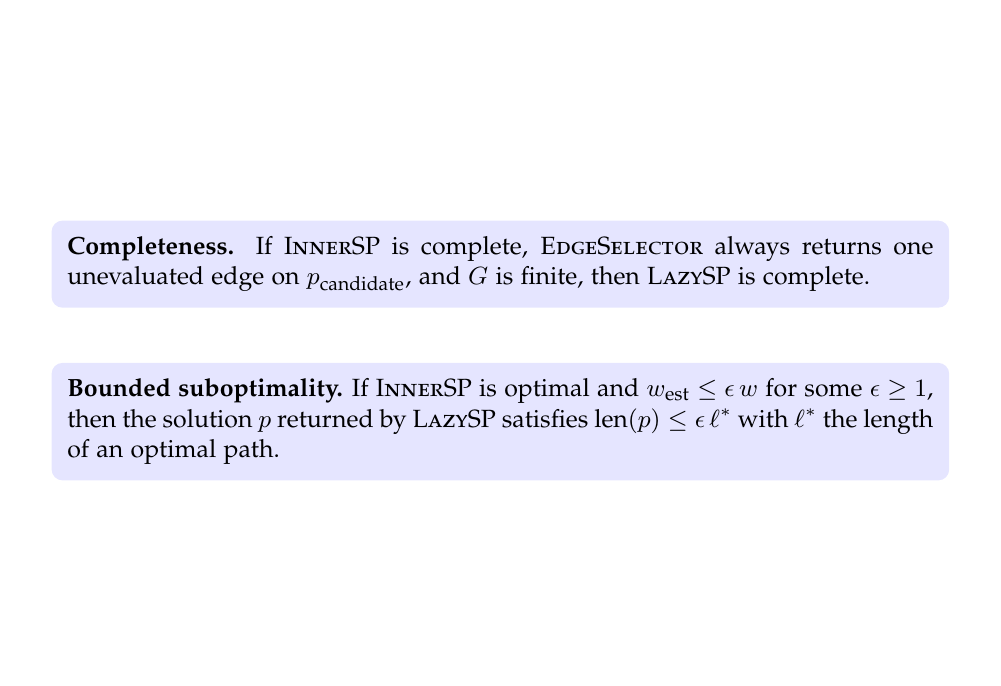
\begin{tikzpicture}
      \draw[step=1,black!15,very thin,opacity=\gridopacity] (0,0) grid (12,8);
   
      \node[inner sep=0.2cm,fill=blue!10,rounded corners] at (6,5) {\begin{minipage}{11cm}\small{
         \textbf{Completeness.} If {\sc InnerSP} is complete,
         {\sc EdgeSelector} always returns one unevaluated edge on
         $p_{\ms{candidate}}$,
         and $G$ is finite,
         then {\sc LazySP} is complete.
      }\end{minipage}};
      
      \node[inner sep=0.2cm,fill=blue!10,rounded corners] at (6,3) {\begin{minipage}{11cm}\small{
         \textbf{Bounded suboptimality.}
         If {\sc InnerSP} is optimal
         and $w_{\ms{est}} \leq \epsilon \, w$
         for some $\epsilon \geq 1$,
         then the solution $p$ returned by {\sc LazySP}
         satisfies $\mbox{len}(p) \leq \epsilon \, \ell^*$
         with $\ell^*$ the length of an optimal path.
      }\end{minipage}};
   \end{tikzpicture}
   
\end{frame}


\end{document}
